\chapter{Thematic Analysis Materials}
\label{app:codebook}

This appendix reproduces the reflexive thematic analysis workbook as exported from the project Miro board.

\newpage
\section{Interview extracts board (raw)}
\label{app:thematic-quotes-raw}

\noindent
First page of the full colour-coded transcript extract board.

\begin{center}
  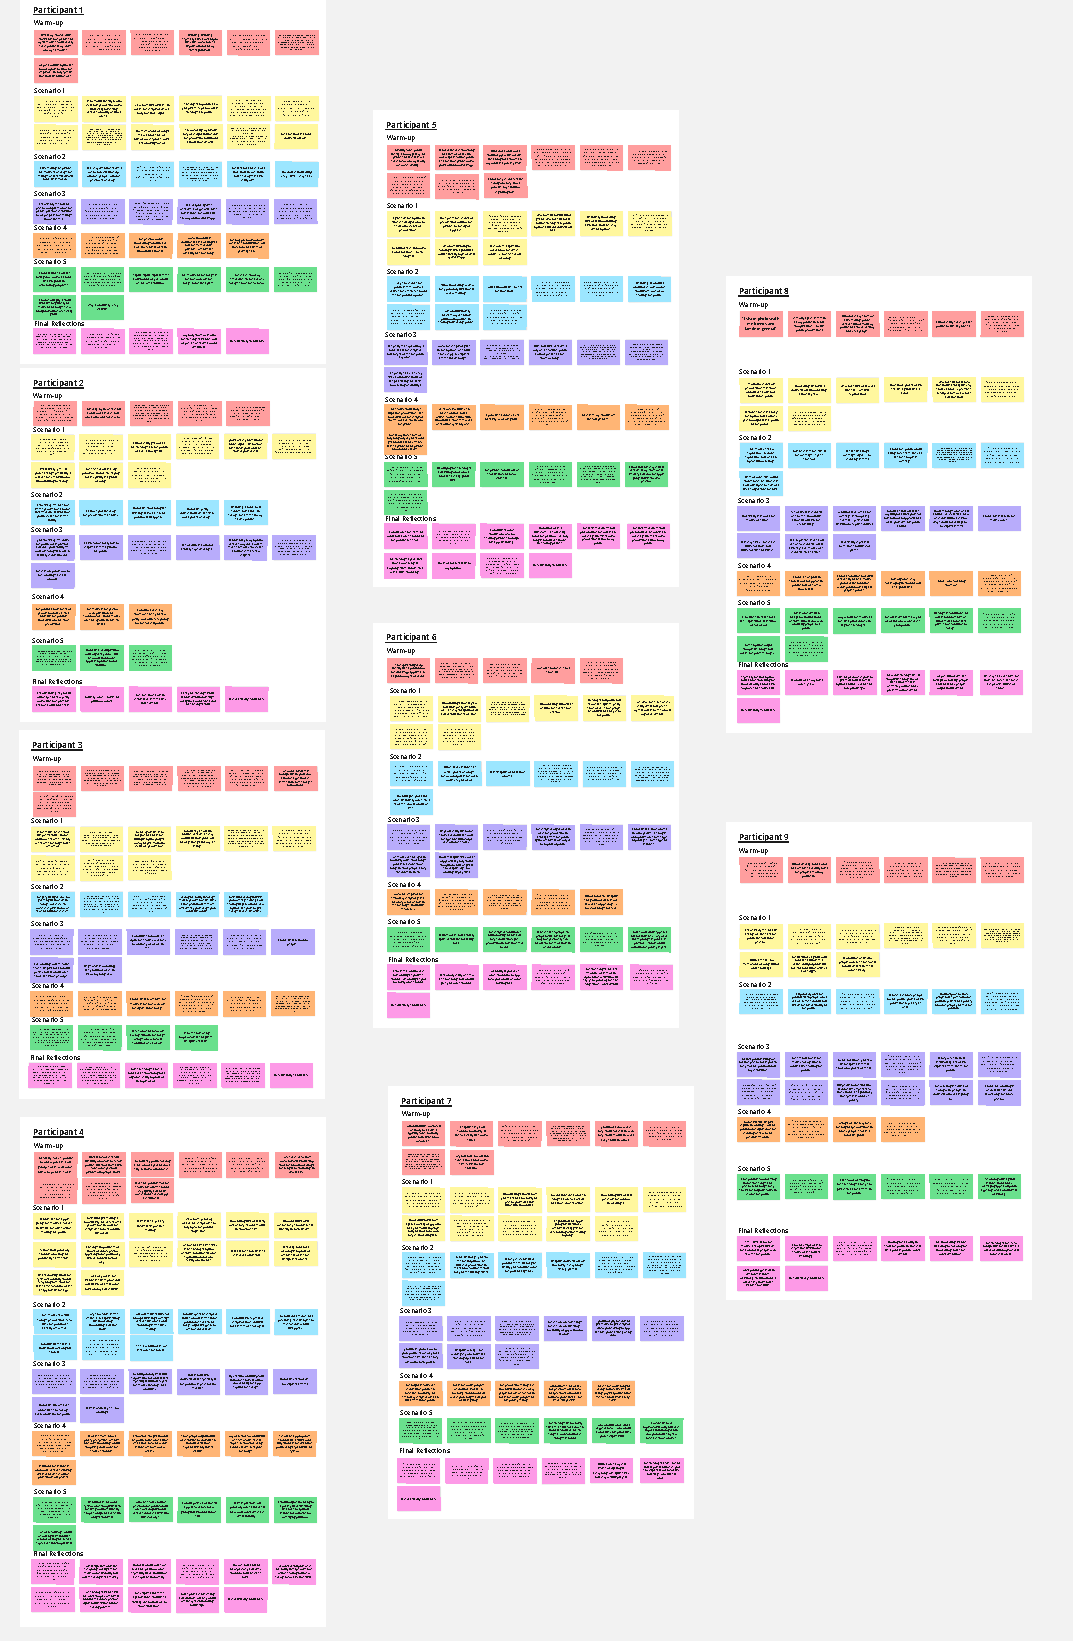
\includegraphics[page=1,width=0.75\textwidth]{appendix-materials/thematic-analysis/interview-extracts-raw-board.pdf}
\end{center}

\newpage
\section{Inductive codebook (initial iteration)}
\label{app:thematic-codebook-initial}

\noindent
First page of the initial 56-code codebook produced through close reading of the interview transcripts.

\begin{center}
  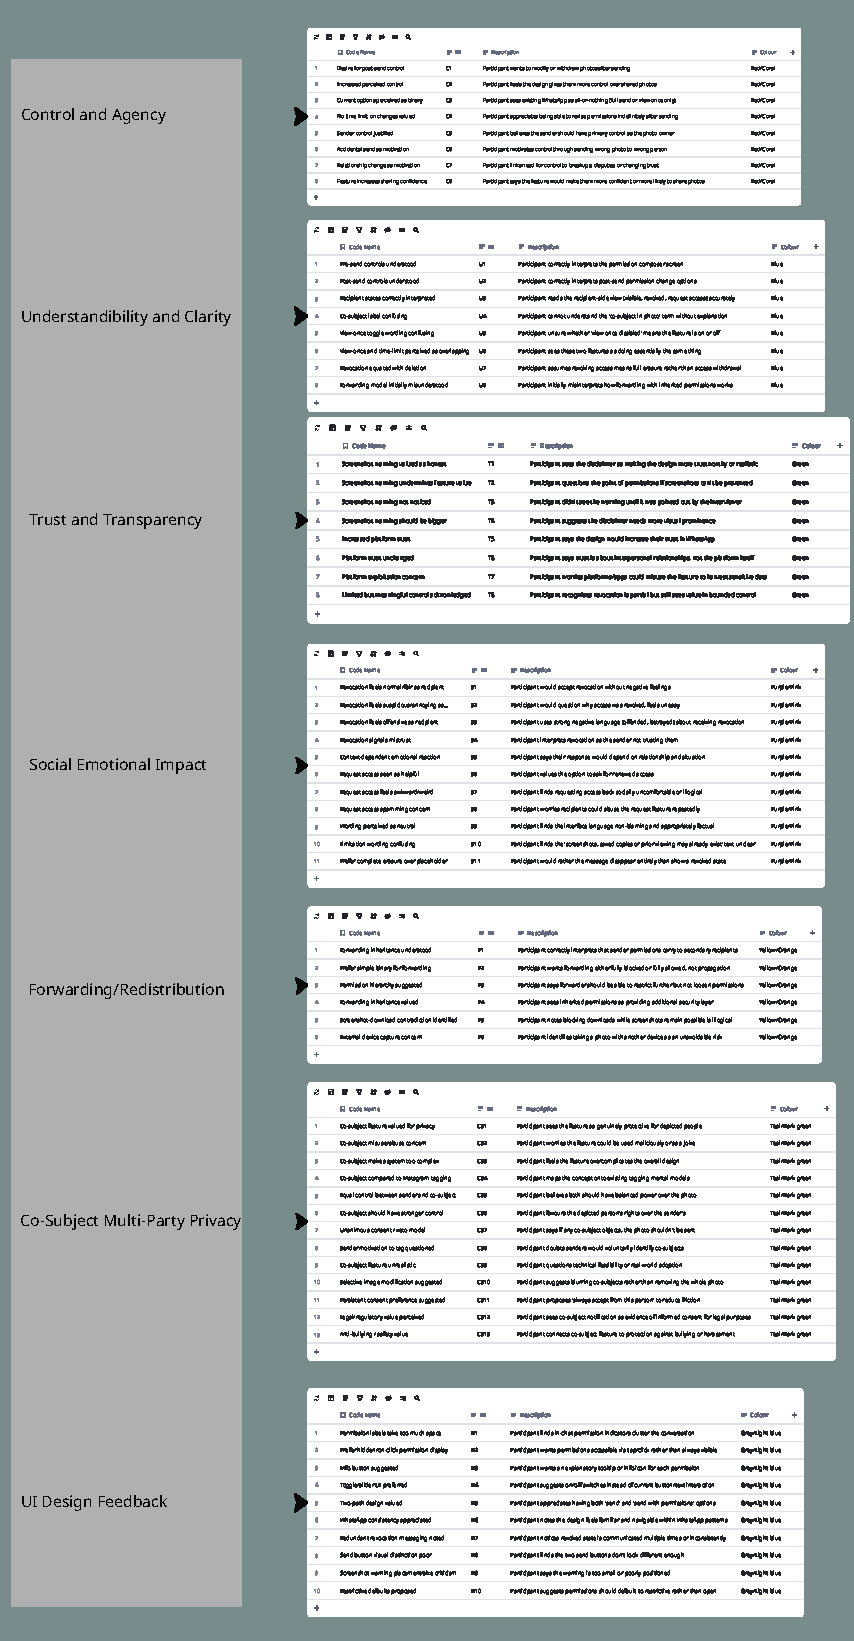
\includegraphics[page=1,width=0.75\textwidth]{appendix-materials/thematic-analysis/inductive-codebook-initial.pdf}
\end{center}


\section{Interview extracts (refined subset)}
\label{app:thematic-quotes-refined}

\noindent
First page of the refined extract set used for focused coding.

\begin{center}
  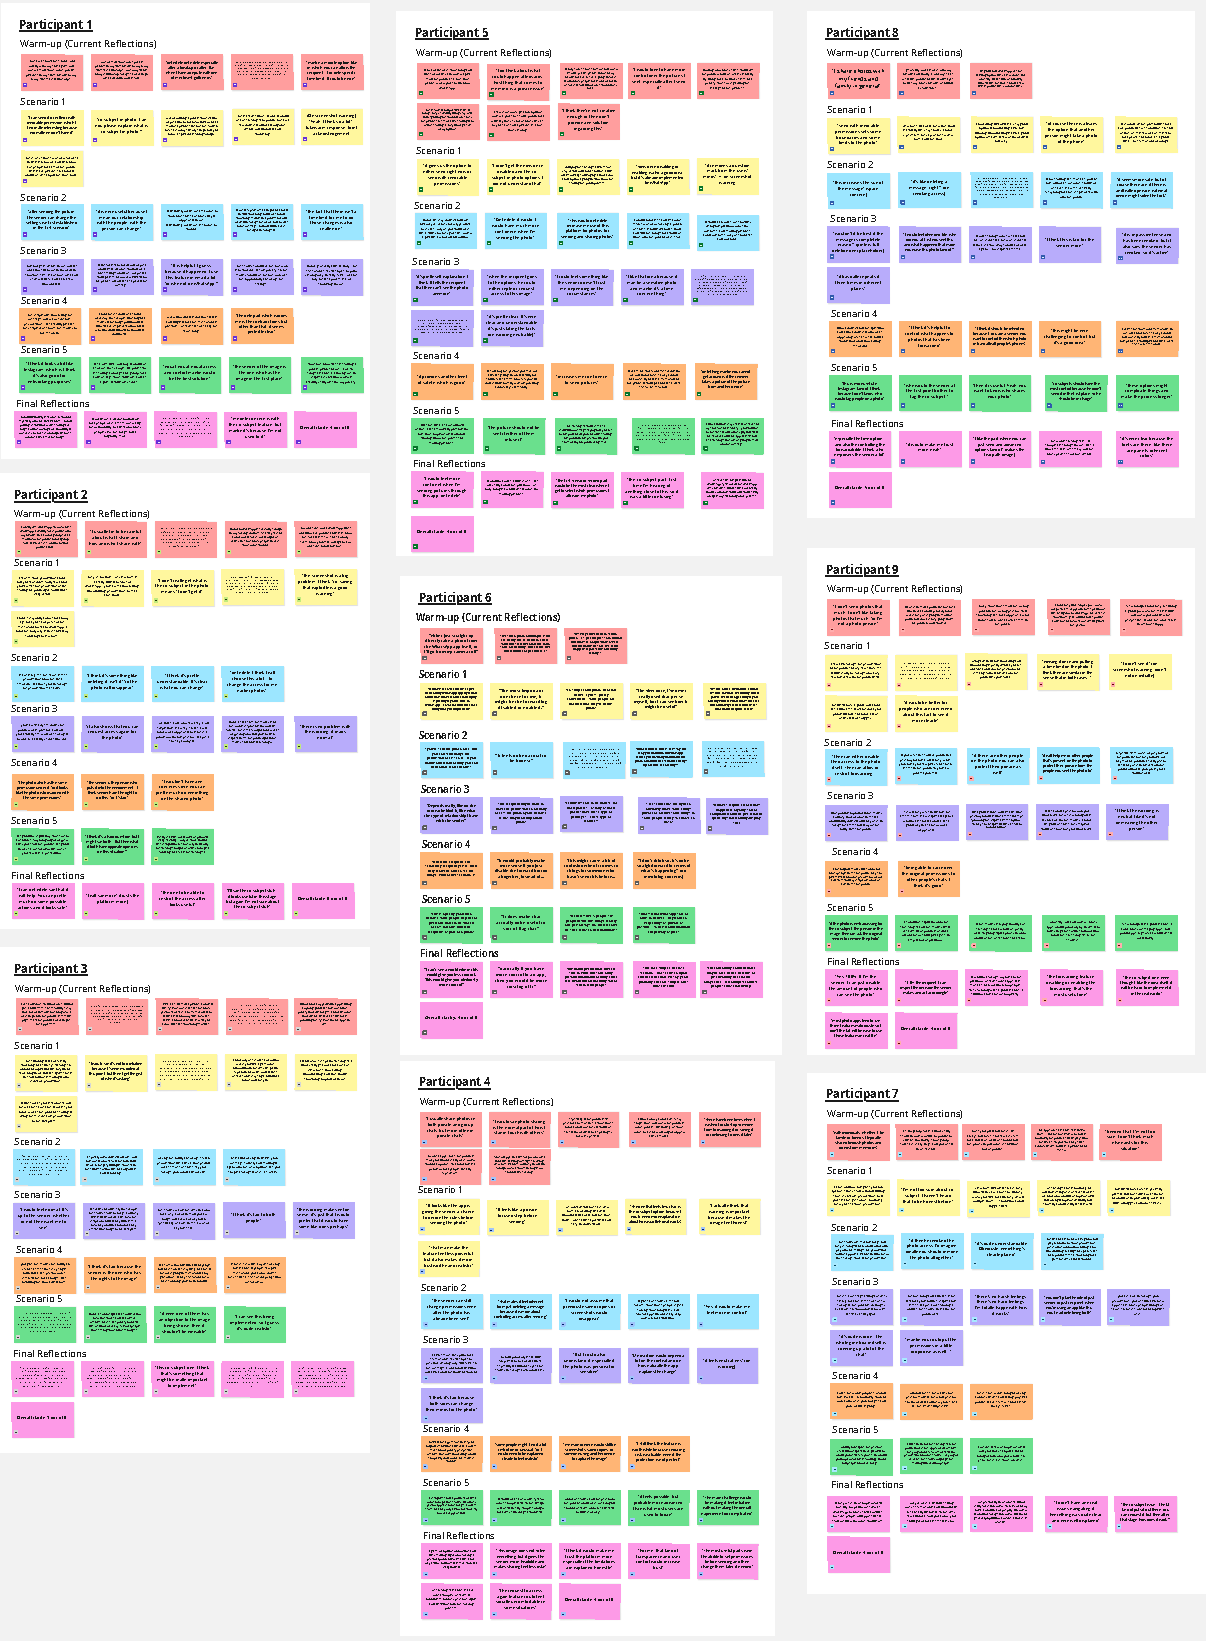
\includegraphics[page=1,width=\textwidth]{appendix-materials/thematic-analysis/interview-extracts-refined.pdf}
\end{center}

\newpage
\section{Working codebook (simplified)}
\label{app:thematic-codebook-working}

\noindent
First page of the simplified 20-code working codebook used for cross-case tagging.

\begin{center}
  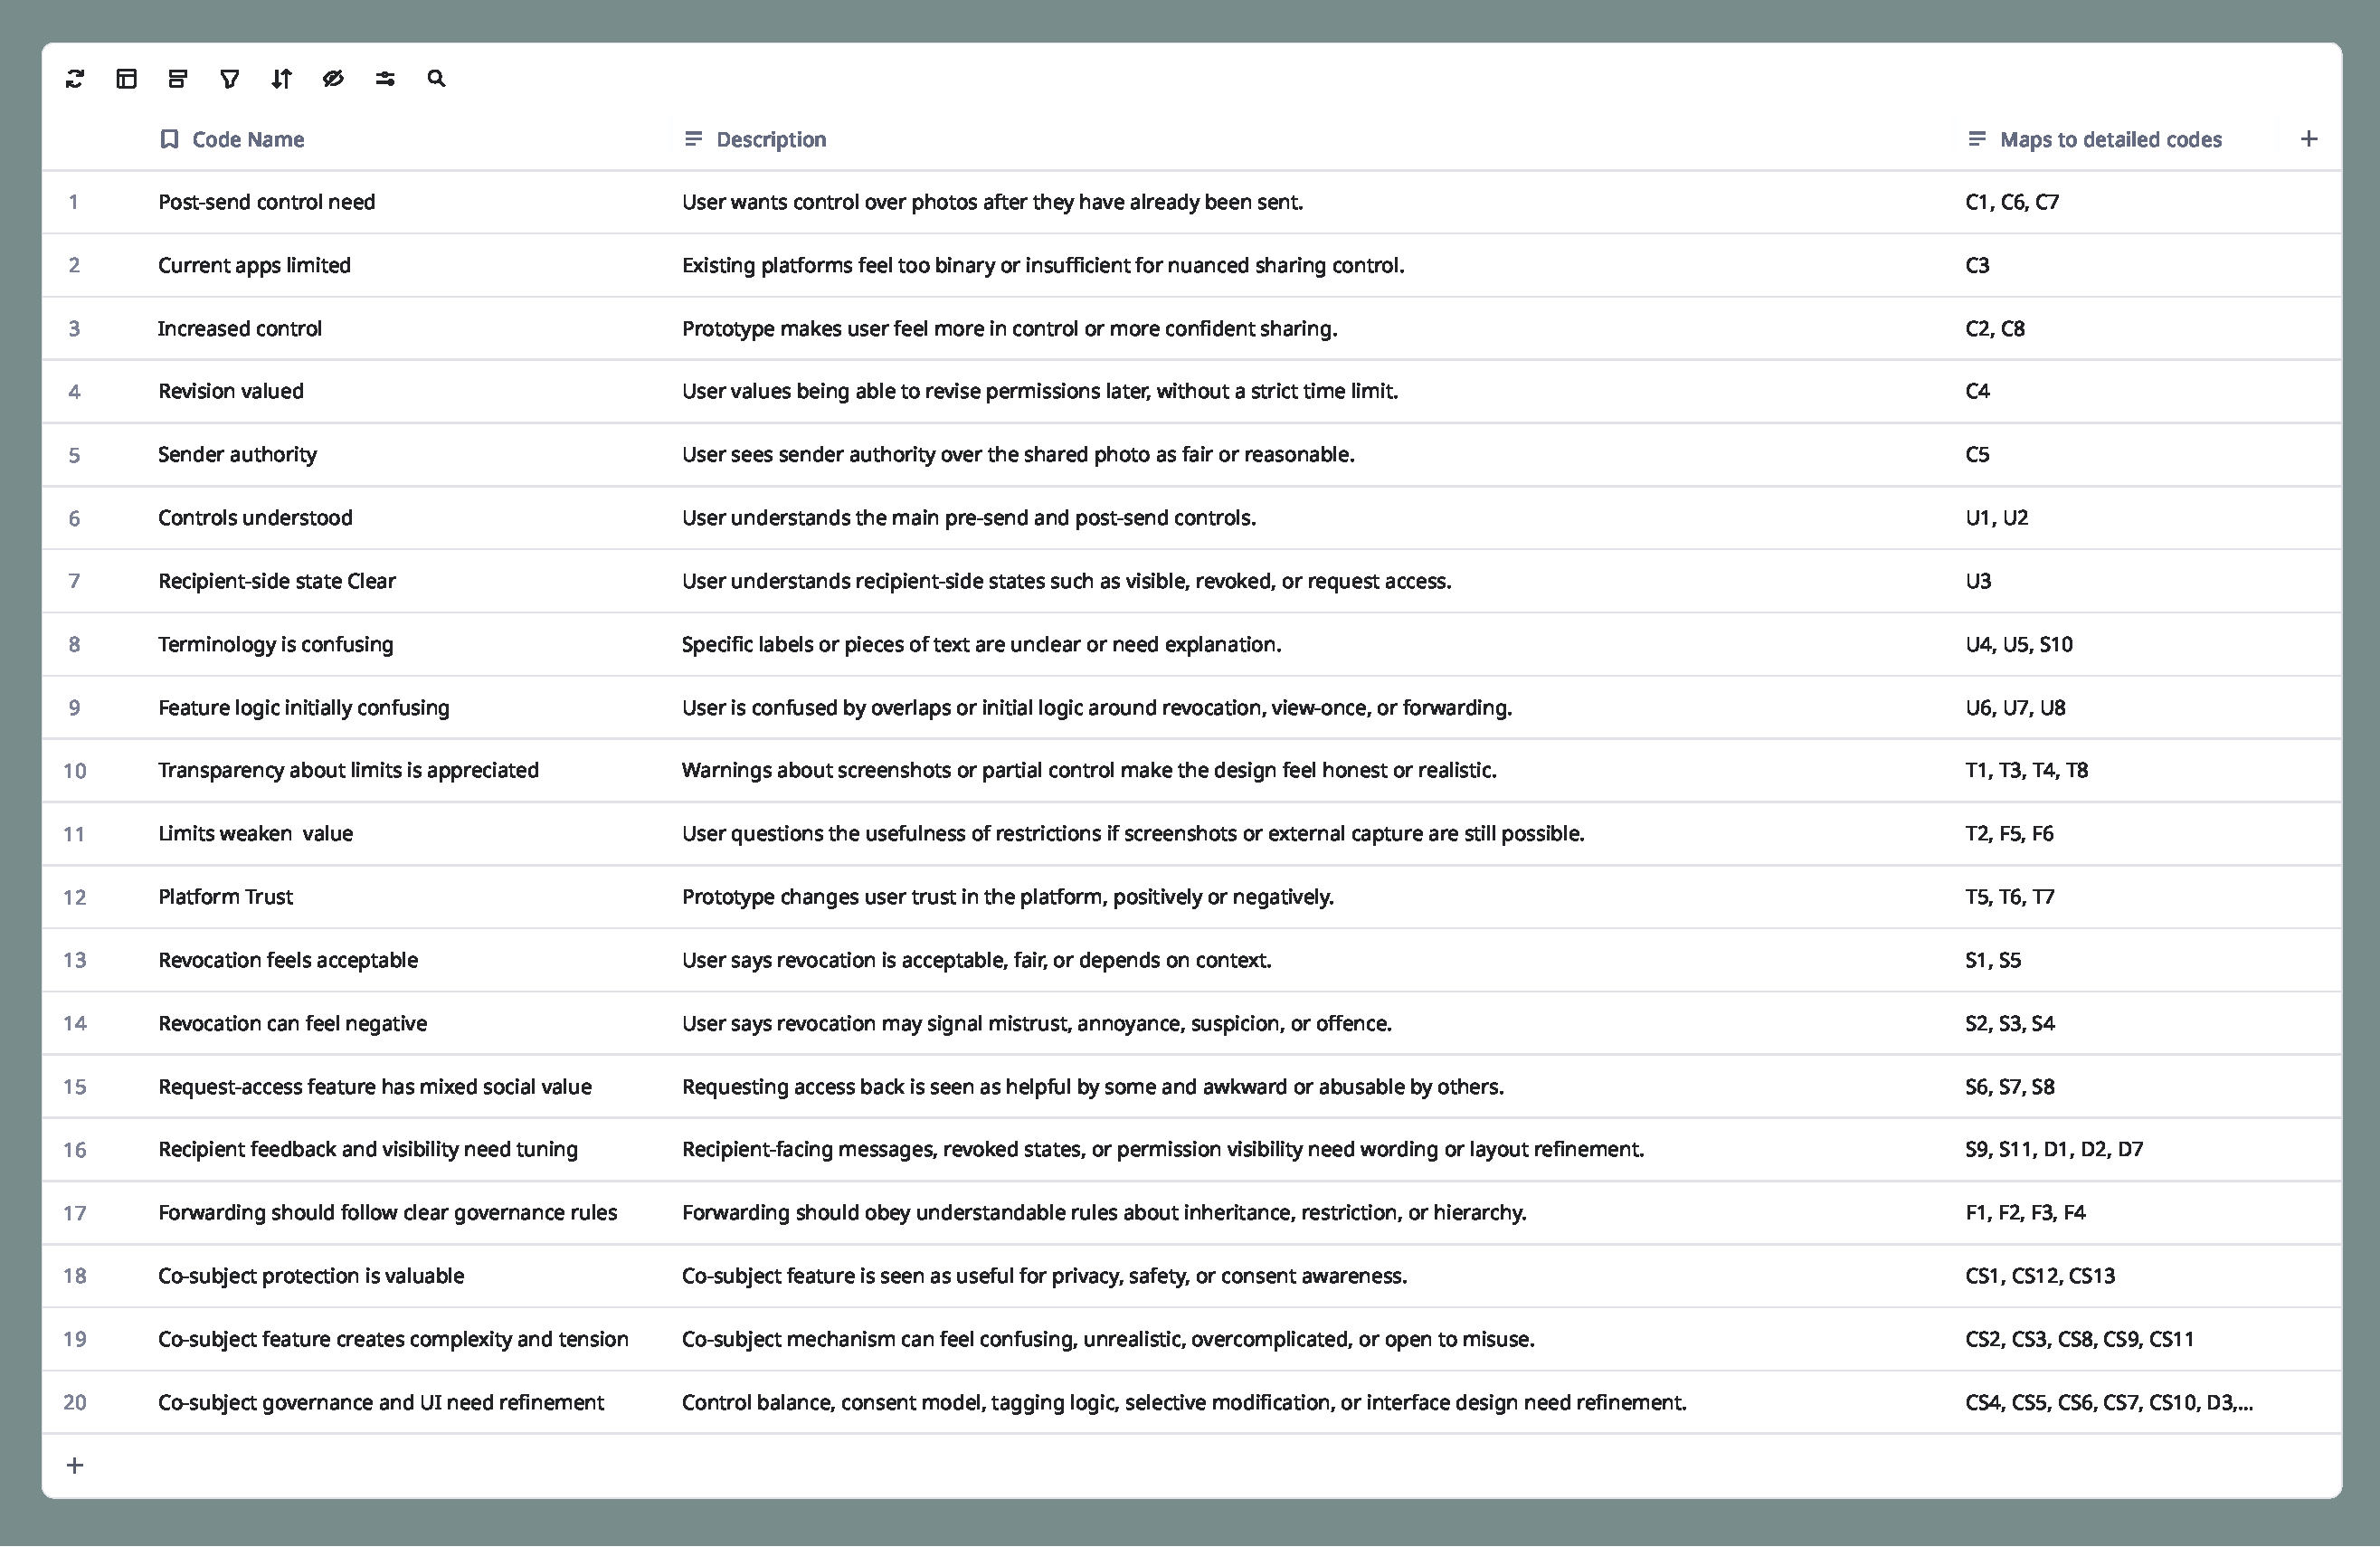
\includegraphics[page=1,width=\textwidth,height=0.88\textheight,keepaspectratio]{appendix-materials/thematic-analysis/working-codebook-simplified.pdf}
\end{center}

\newpage
\section{Quote-to-code coding sheet}
\label{app:thematic-coding-sheet}

\noindent
First page of the quote-to-code mapping sheet.

\begin{center}
  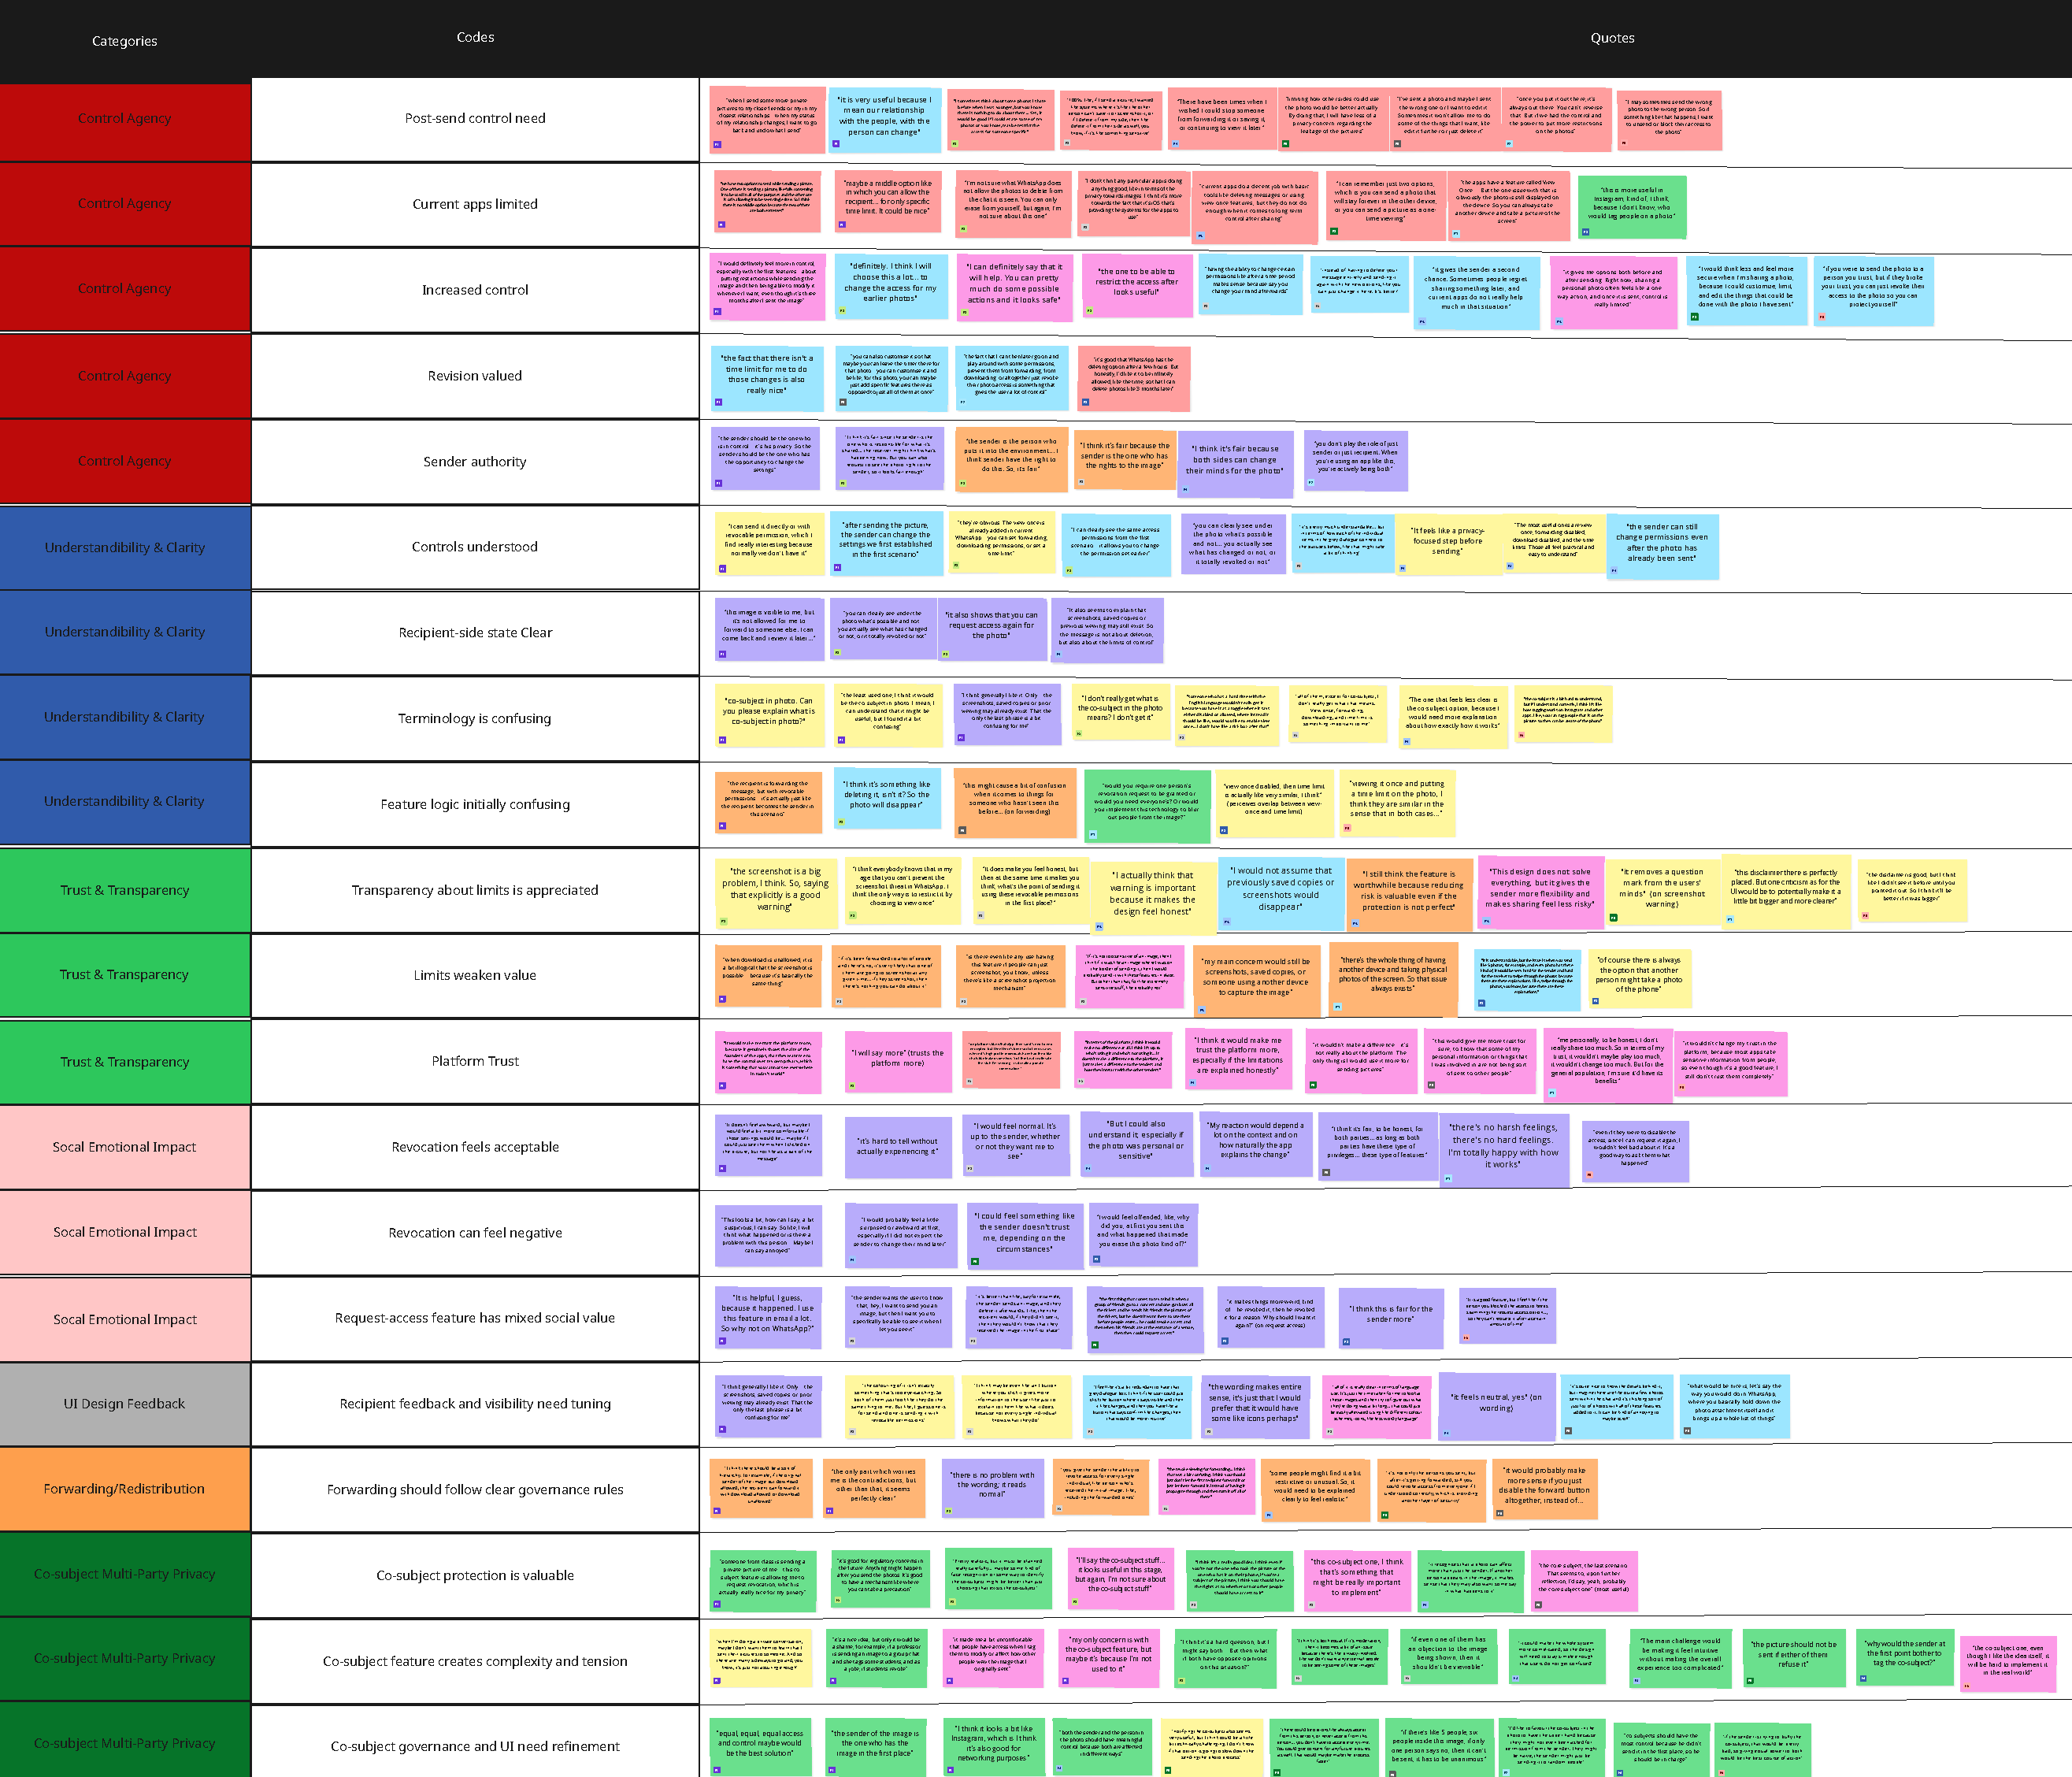
\includegraphics[page=1,width=\textwidth,height=0.88\textheight,keepaspectratio]{appendix-materials/thematic-analysis/quote-to-code-coding-sheet.pdf}
\end{center}

\newpage
\section{Final themes table}
\label{app:thematic-themes-table}

\noindent
First page of the consolidated themes table (definitions, codes, and example quotations).

\begin{center}
  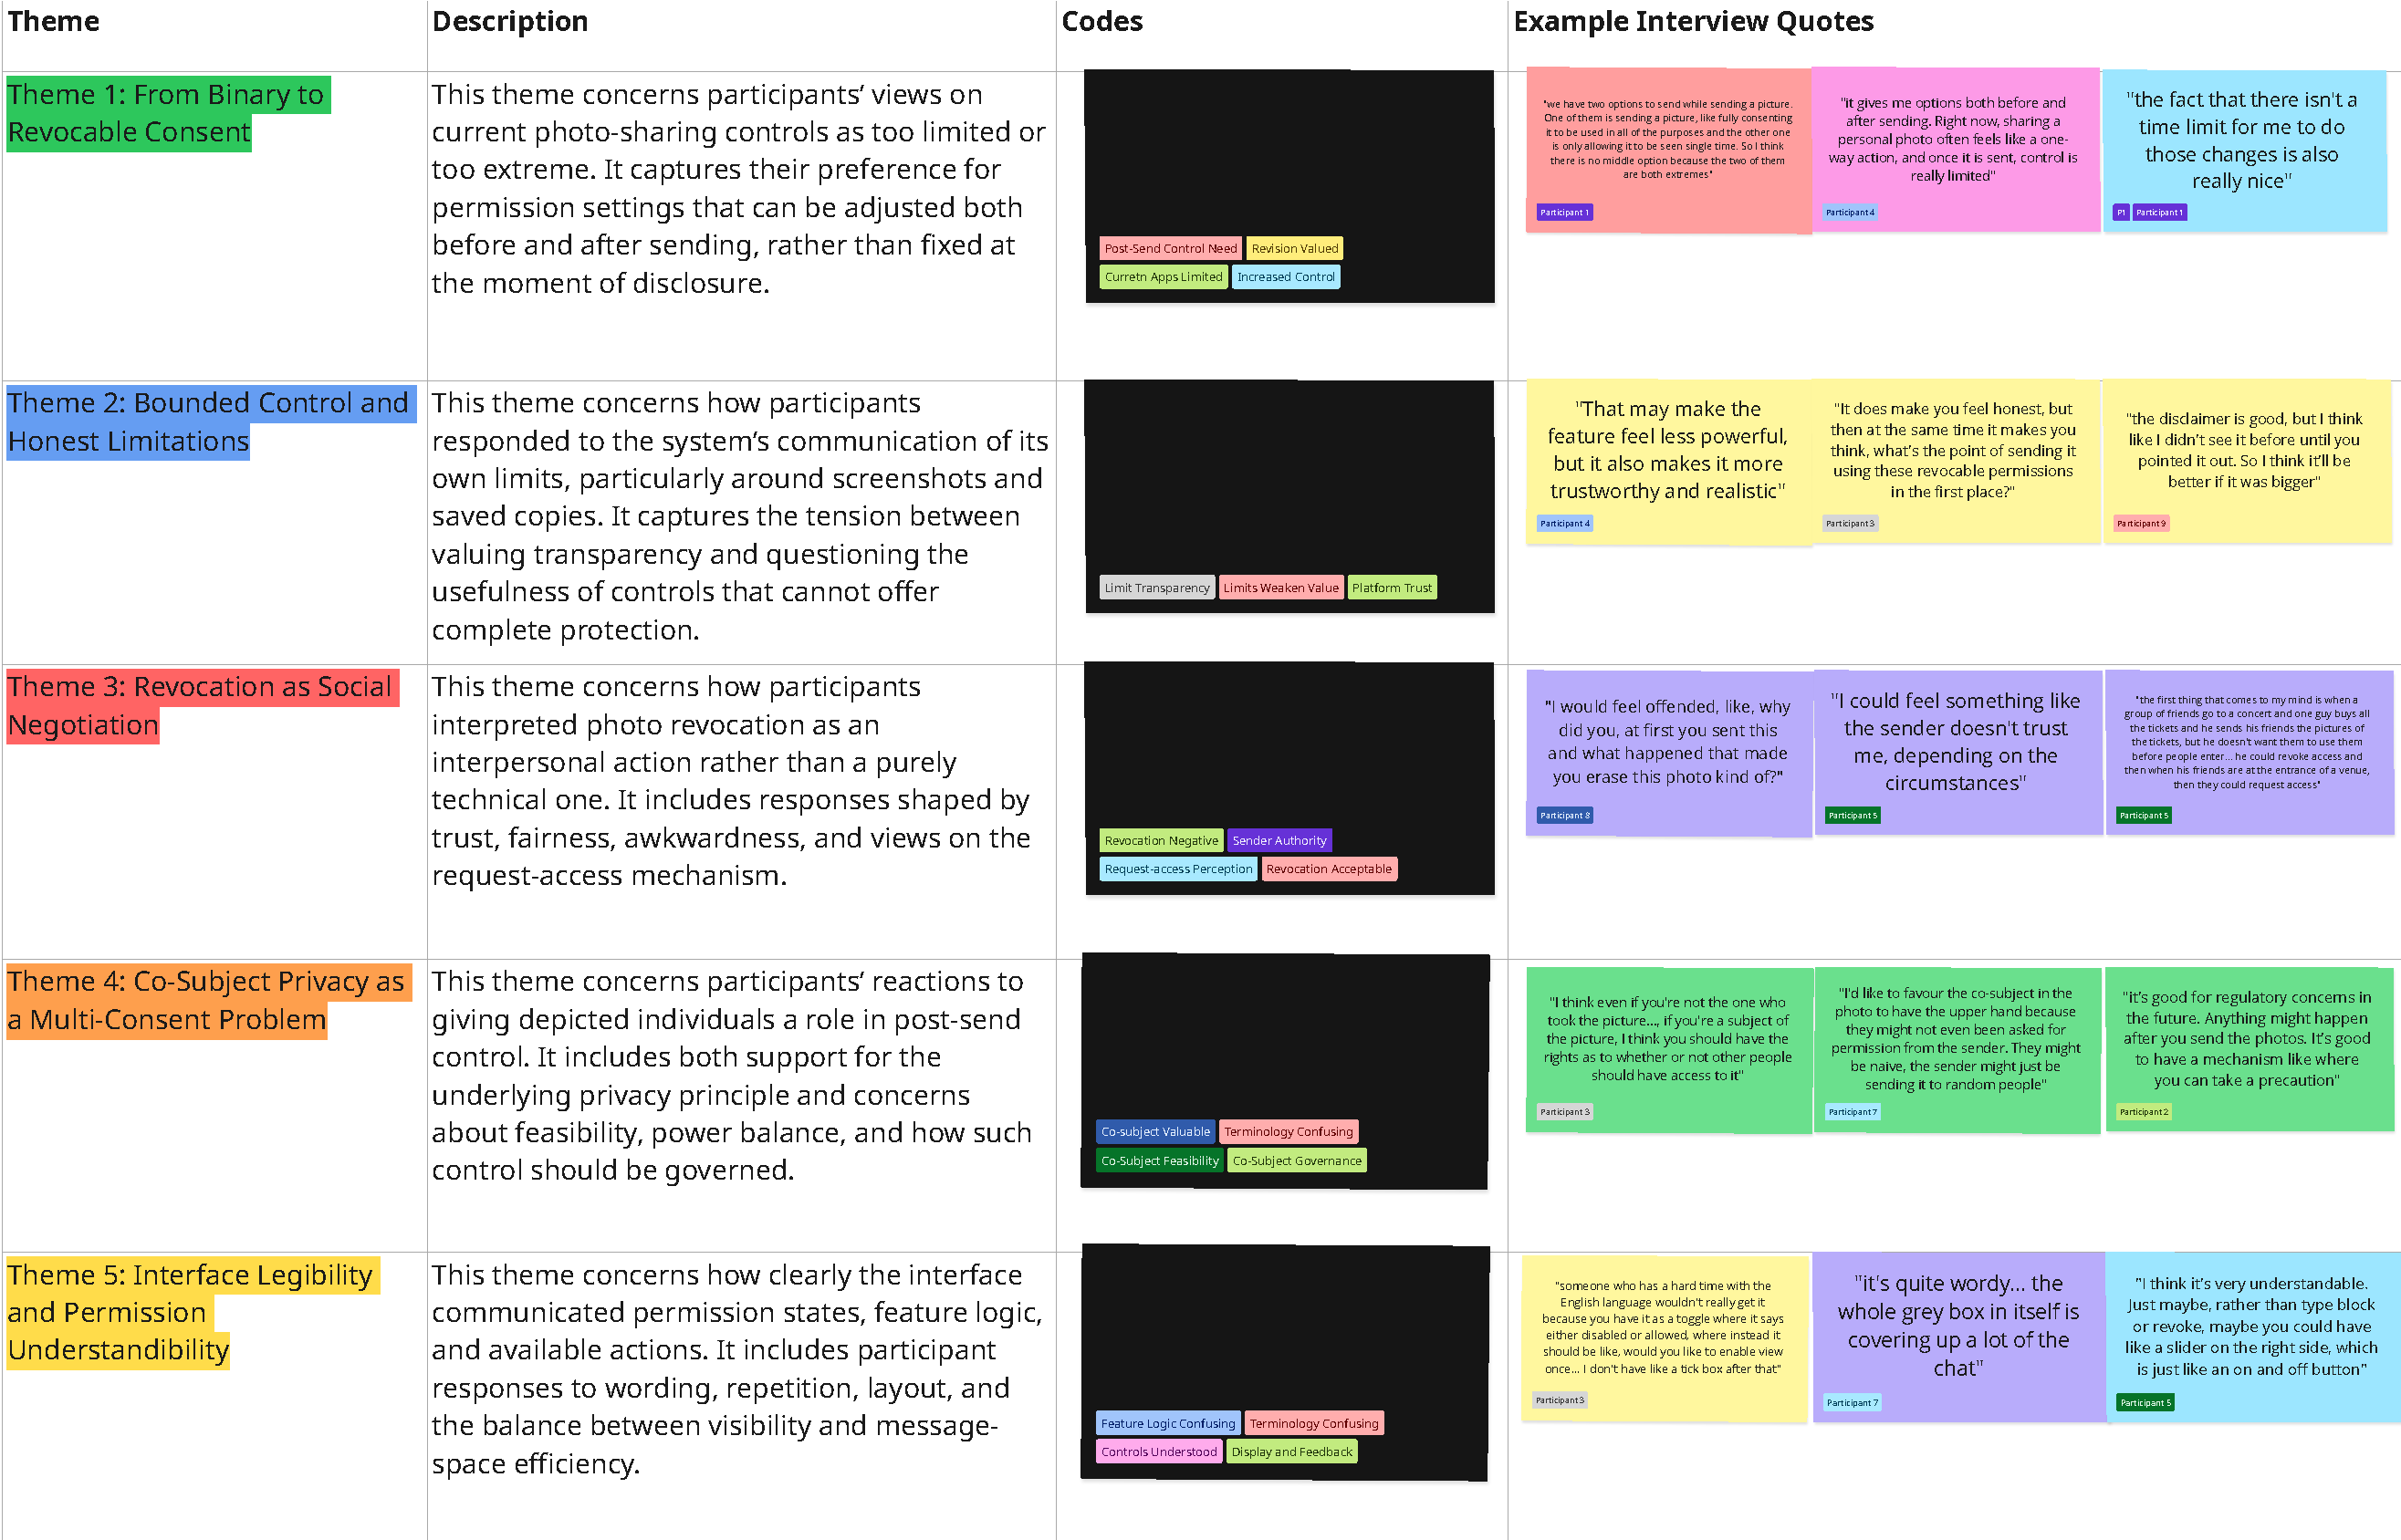
\includegraphics[page=1,width=\textwidth,height=0.88\textheight,keepaspectratio]{appendix-materials/thematic-analysis/final-themes-table.pdf}
\end{center}







